\documentclass[11pt, rgb, bibtotoc, twoside]{scrreprt}

\usepackage{themeKonstanz} 

\usepackage{lipsum}

\format{a4}

% Thesis information  %
\year{2024}
\author{Fabian Klopfer, M.Sc.}
\title{Extraction of Quantitative Relaxation and Diffusion Metrics from balanced Steady-State Free Precession Magnetic Resonance Imaging}
%Multi-dimensional Feature Extraction of Quantitative Relaxation and Diffusion Brain Magnetic Resonance Imaging
\uni{University of Tübingen}
\unisection{Faculty of Science \\ Faculty of Medicine}
\department{Graduate School of Neuroscience}
\institute{Department for High-field Magnetic Resonance \\ Max Planck Institute for Biological Cybernetics}
\supervisorOne{Dr. Rahel Heule}
\supervisorTwo{Prof. Dr. Klaus Scheffler}

\headFoot{14}
 
\bibliography{resources} 

\begin{document}
\thesistitlepage[language=english]

\begin{abstract}
\begin{center}
    \textbf{Abstract:}
\end{center}{}
\lipsum[1]
\end{abstract}


\newgeometry{left=2.5cm, right=2.5cm, bottom=2cm, top=2.5cm, headheight=14pt, headsep=0.8cm, footskip=30pt}
\tableofcontents


\restoregeometry
\rmfamily 
\normalsize

\chapter{Introduction}
\begin{itemize}
 \item Largest multi modal data set of its kind
 \item bSSFP now feasible with new HW
 \item Speeds up scanning times potentially yielding multiple modalities with one scan
 \item Limited data available for ML applications
\end{itemize}

\cleardoublepage
\chapter{Background \& Related Work}
In this chapter, relevant background knowledge and related previously published work is discussed.

\section{Magnetic Resonance Imaging}
\subsection{Fundamentals of MRI}
%% RAD 229 Lect-01 A
MRI uses the ability of certrain nuclei to absorb and emit energy in the radio frequency spectrum to generate images of organisms.
This ability is called Nuclear Magnetic Resonance and depends on charge, spin, and mass, which are the intrinsic properties of particles. \\
\textbf{Nuclear Magnetic Resonance-active Nuclei} are those atoms with  with an odd number of protons and/or neurtons\autocite{nishimura, halliday}.
They have a spin angular momentum defined as
\[ S = \hbar I, \]
where $I$ is the spin operator and $\hbar$ is Planck's constant normalized by $2\pi$.
The odd number of protons/neutrons also induces a magnetic dipole moment
\[ \mu = \gamma S. \]
$\gamma \ [\text{MHz} / \text{T}]$ is called the gyromagnetic ratio and is unique to each nuclear magnetic resonance-active nuclei.
It is the ratio of the magnetic dipole moment $\mu$ to the spin of a particle $S$.
The gyromagnetic ratio governs the frequency of precession and is meassured empirically. \\
Specifically, ${}^1$H has a spin of $0.5$, a high natural abundance of $0.998$ and is therefore used primarily for clinical and medical MRI.
its gyromagnetic ratio is $\gamma = 42.57$ MHz$/$T.\\
When placing such nucleie into a magnetic field, the spins have a tendency to align with its direction, leading to a net or bulk magnetization per unit volume (or voxel) $v$,
\[ M = \sum_{v \in V} \mu_v. \]
Additionally, due to spin and mass, the nucleus exhibits an angular momentum, i.e. it precesses e.g. in a gravitational field.
The dynamics of this angular momentum  or pecession can be described by
\[ \frac{d \mu}{d t} = \mu \times \gamma B, \]
when considering a single nucleus and for a summing over a unit volume
\[ \frac{d M}{d t} = M \times \gamma B. \]
The combination of magnetic and angular momentum causes the nucleus to precess in a magnetic field as well with a specific frequency --- called the Larmor frequency:
\[ \omega = \gamma B, \]
where $B \ [T]$ is the strength of a magnetic field and $\gamma$ is the gyromagnetic ratio.

A scanner MR scanner consists of a primary electromagnetic coil, that is surrounded by a cryostat and thermal insulation, an excitation coil, spatial localization coils, and a receiver coil, as shown in \ref{scanner-teardown}.
The excitation and the receiving coil are merged into one RF coil here. \\
\fig{img/mri-scanner_teardown.png}{scanner-teardown}{MRI scanner with a part cut-away such that the main components are visible~\autocite{MRIAGuidedTourMagnetAcademy-2024-05-07}.}{0.5}

This \textbf{primary electromagnet} provides the main magnetic field $B_0$ to polarize the NMR-active nuclei with field strengths up to $14.2 T$, but usually about $1.5 T$ to $3 T$ in medical applications.
This is several orders of magnitude larger than the earth magnetic field which is approximately $0.5$ Gauss
To provide such high fields, super-conductivity needs to be reached, thus the coil is cooled using liquid helium.
The $B_0$ field is spatially uniform and temporally stable in an ideal scanner, such that the same polarization is applied to all atoms.
In practice this field is not perfectly homogeneous, such that magnetic field probes are used to measure the field and shim cards are used to correct these inhomogenieties.
This is called passive shimming.
Alternatively, active shimming coils can be used to smooth the inhomogenieties.
It is oriented along the ``long'' part of the scanner, so if a human lies in the scanner, the poles are oriented towards the head and the feet of the subject.
We call this axis the $z$-axis. \\

%% RAD 229 Lect 01 B
Additionally, an \textbf{excitation system} is necessary to generate exciting magnetic pulses $B_1(t)$ to cause nutation of the nuclei of interest as well as to refocussing, spoiling, inversion and saturation.
The $B_1(t)$ field is a radio frequency field with the excitation frequency defined by the $B_0$ field strength, the Larmor frequency of the excitation target nuclei and are both short in duration and amplitude.
For example with $B_0 = 3$T we get
\[ 42.58 \frac{\text{MHz}}{\text{T}} \cdot 3 \text{T} = 127.74 \text{MHz}. \]
Typical pulse durations are on the intervall $[0.1, 10]$ ms and amplitude about $< 25 \mu \text{T}$.
The shape of the excitation pulse is governed by an envelope function in terms of amplitude trajectory.
\fig{img/nutation.png}{nutation}{A visualization of rotation $r$ (in out case we call it spin) in green, precession p in blue --- at the Larmor frequency --- and nutation n in red~\autocite{FilePraezessionsvgWikimediaCommons-2024-04-23}.}{0.2}
The excitation pulses are perpendicular to the $B_0$ field, which is important to enable the excitation pulses to tip the spin system in the presence of the strong polarizing field.
While the $B_0$ field causes polarization, thus alignment and precession, the $B_1(t)$ pulses cause a ``tipping'' or nutation of the precession --- shown in \ref{nutation}, generating transverse magnetization such that it is detectable using Faraday's law of induction.
An example of an excitation pulse is
\[ B_1(t) = B_1^e (t) \left(\cos\left(\omega_{RF} t + \theta \right) i - \sin\left(\omega_{RF} t + \theta \right) j \right), \]
with $B_1(t)^e (t)$ a pulse envelope function, e.g. \texttt{sinc} or \texttt{rect} functions, $\omega_{RF}$ the excitation carrier frequency which should match the Larmor frequency of the spin system, and $i, \ j$ the polarization directions.
Additionally a RF pulse has a filp angle $\alpha$ which is the angle between the $z$-axis and the $B1$ pulse (called inclination in spherical coordinates) and a phase $\theta$ which is the angle in the $xy$ plane, starting at the $x$-axis (azimuth in spherical coordinates).
The excitation system is commonly implemented using a birdcage coil as it's highly efficient in terms of energy, excitation and  heating mitigation.
The $B_1(t)$ field is supposed to be highly uniform, especially radially while decaying slightly axially. \\

A \textbf{receiving coil(s)} reads out the response of the excited tissue.
This can be the same RF coil that is used for excitation.
As the precessing magnetization causes induction in the receiving coil(s), the flux in the receiving coil changes causing an electromotive force
\[ \epsilon = - \frac{\partial \Phi}{\partial t}. \]
The picked up signal is further split up, multiplied by $\cos{\omega_0 t}$ and $\sin{\omega_0 t}$ respectively and low-pass filtered to get the in-phase signal $I(t)$ and the quadrature signal $Q(t)$.
The These signals are then quantized, yielding $I(t)$ as the real and $Q(t)$ as the imaginary part of the signal.

The excitation forces the magnetization off from its equilibrium state and thus induces relaxation back to the equilibrium again after excitation.
This relaxation can be separated into two components: longitudinal and transverse relaxation.

The longitudinal component can be described as a return to the equilibrium state of the magnetization on the $z$-axis
\[ \frac{d M_z}{d t} = - \frac{M_z - M_e}{T_1}, \]
where $M_e$ is the equilibrium nuclear magnetization, which is proportional to the applied magnetic field $B_0$~\autocite{nishimura}.
The solution to this equation is
\[  M_z = M_e + (M_z - M_e) \exp{-t / T_1}. \]
$T_1$ is the time constant of the longitudinal component also called longitudinal relaxation time constant or spin-lattice time constant.
It is proportional to the applied field strength and thus lengthens when $B_0$ is increased in strength.
Practically, it is the time that it takes for $M_z$ to return to $63 \%$ of it's thermal eqilibrium state $M_e$~\autocite{relaxation, lauterbur}.
   \begin{figure}[h]
      \begin{center}
         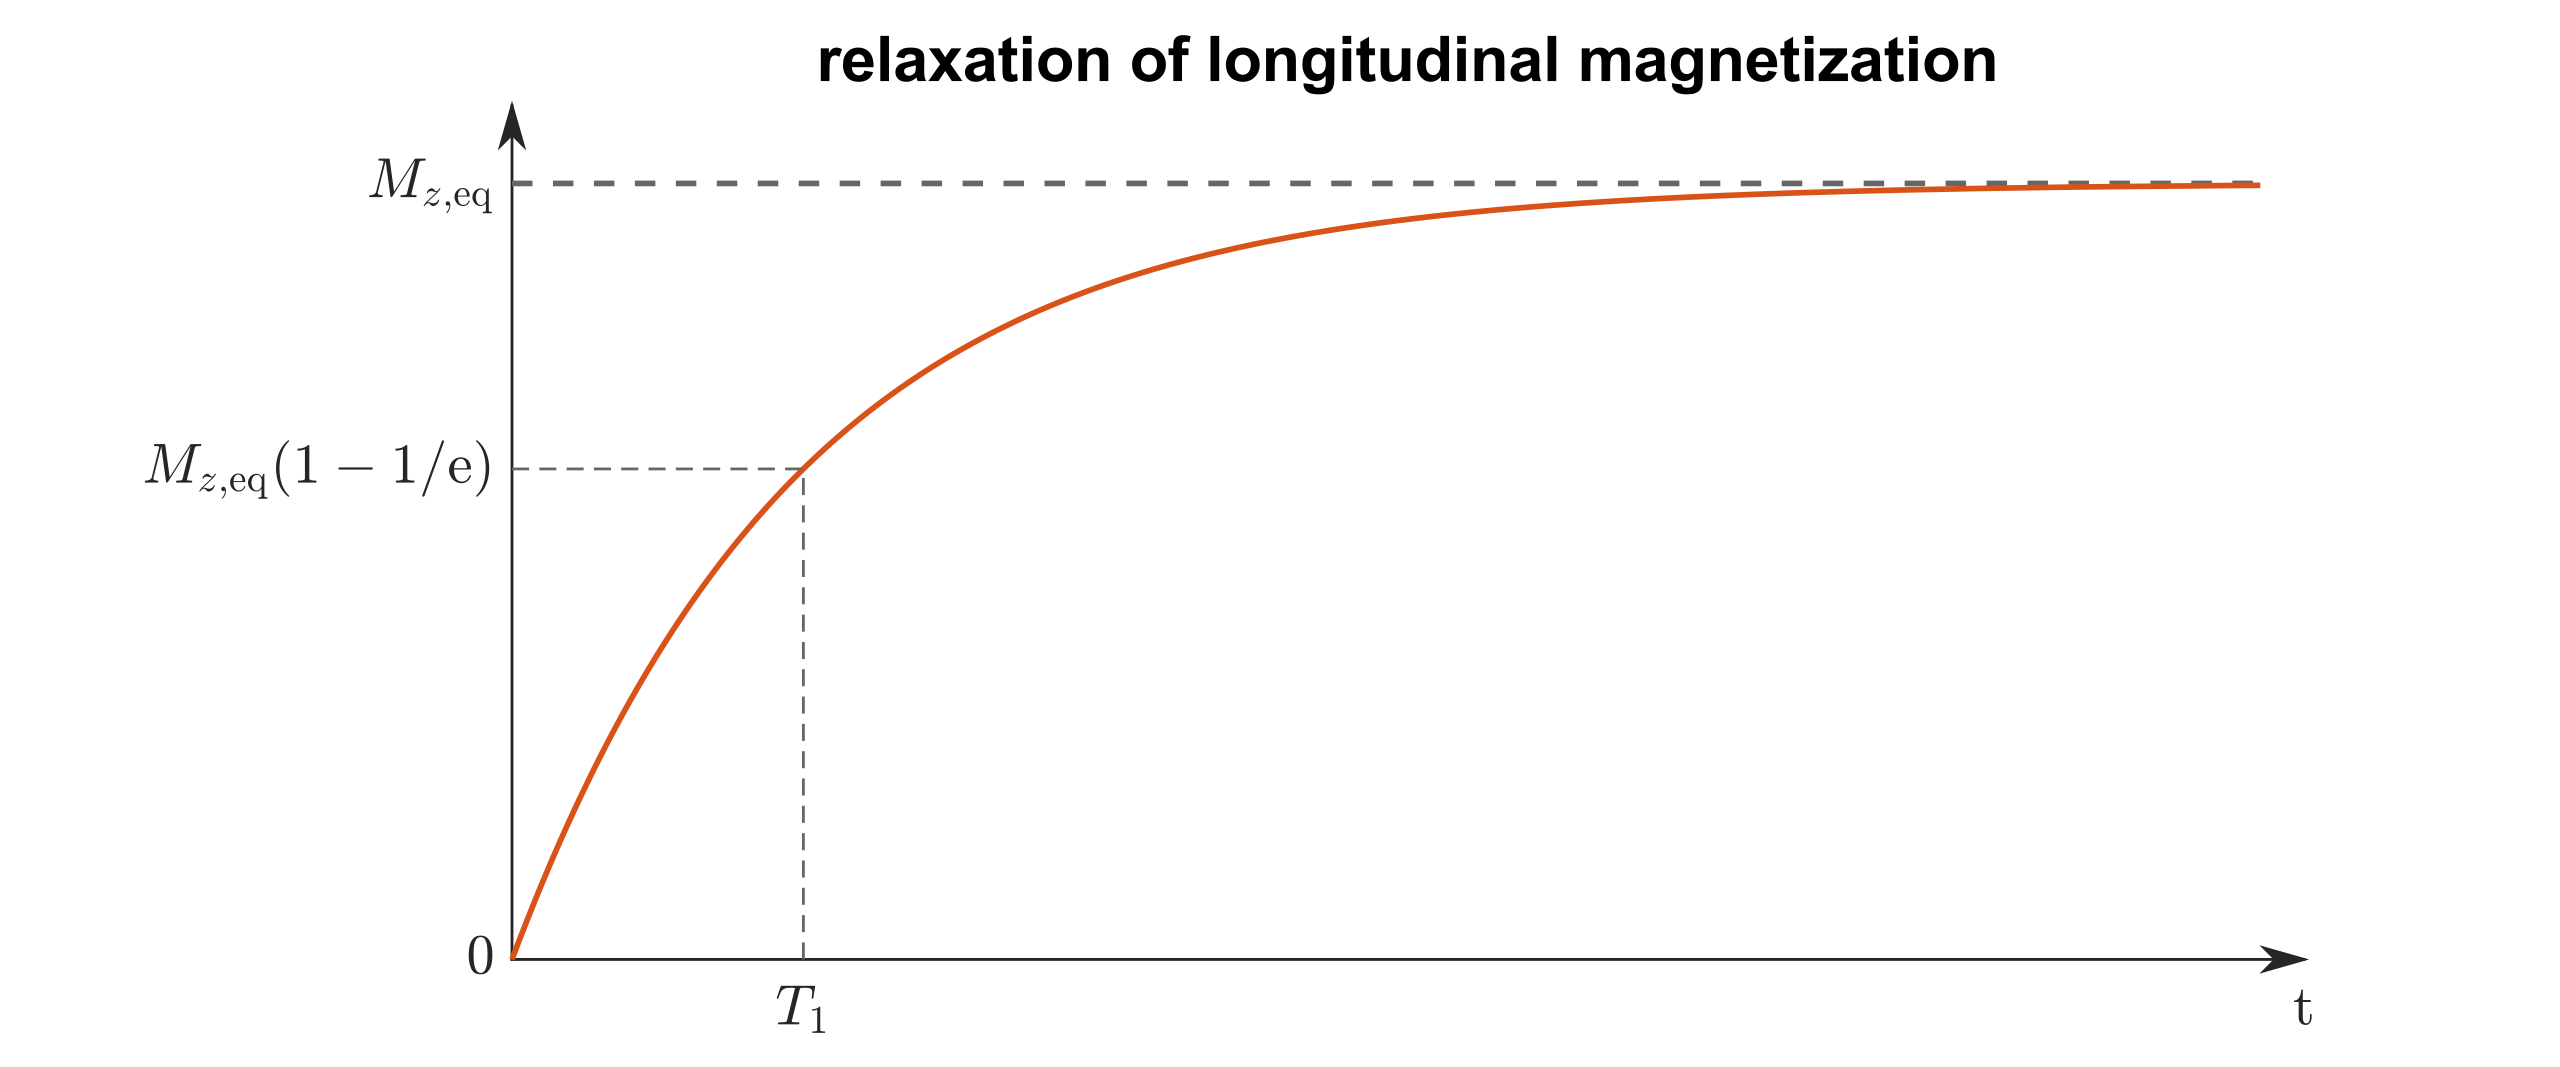
\includegraphics[keepaspectratio, width=0.49\textwidth]{img/t1.png}
         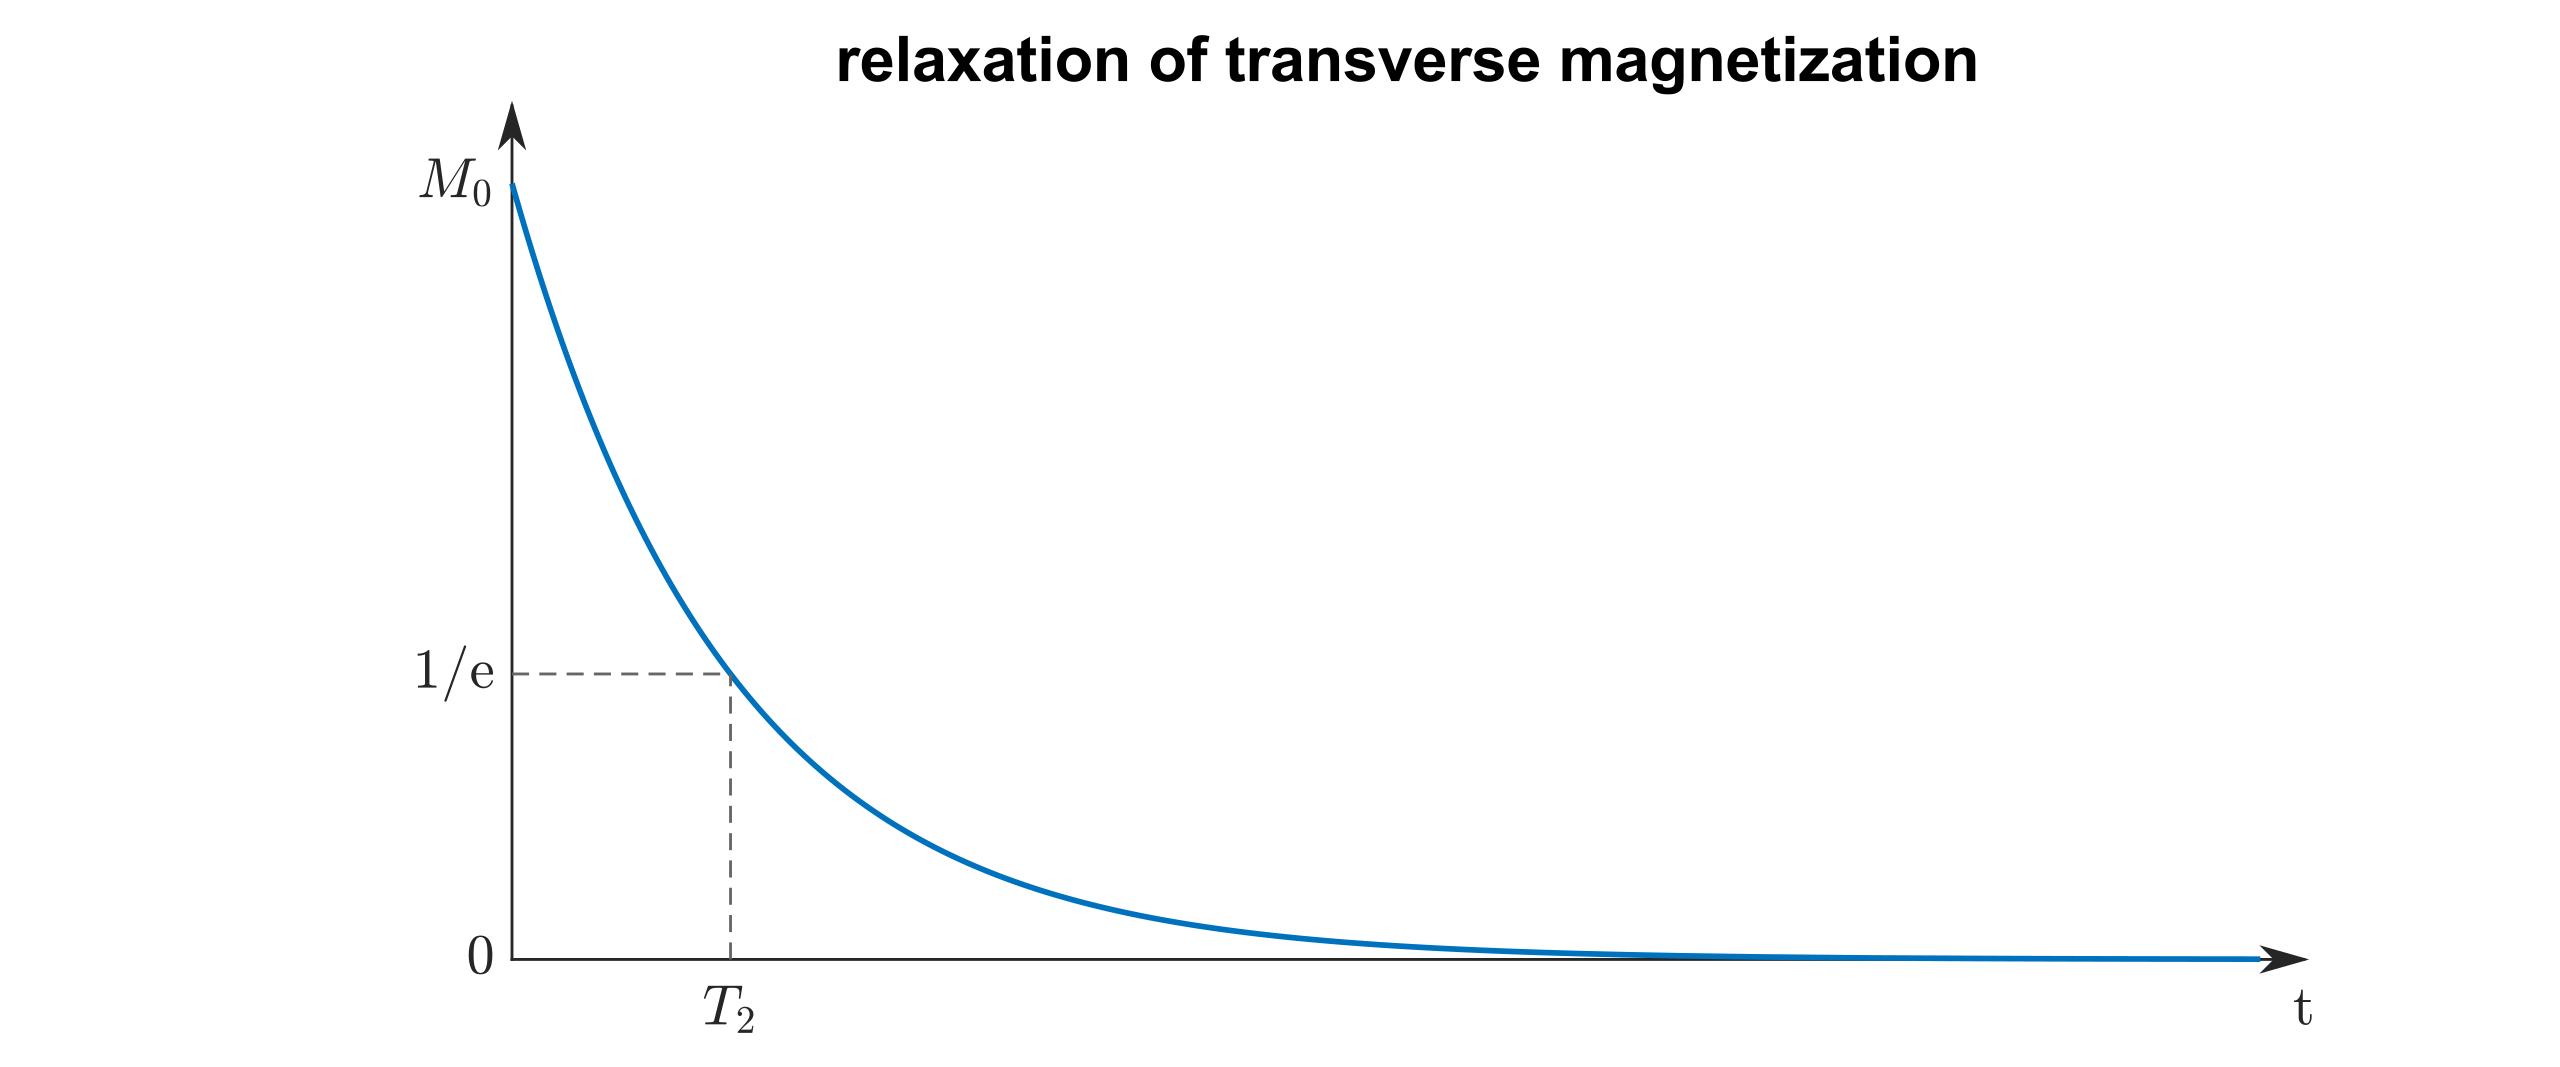
\includegraphics[keepaspectratio, width=0.49\textwidth]{img/t2.png}
      \end{center}
      \caption{
         \textbf{Left:} $T_1$ relaxation curve shows the return to the equilibrium state~\autocite{RelaxationlongitudinalmagnetizationSpinlatticerelaxationWikipedia-2024-05-01}.
         \textbf{Right:} $T_2$ relaxation curve visualizes the transveral magnetization decay to zero~\autocite{RelaxationtransversemagnetizationSpinspinrelaxationWikipedia-2024-05-01}.
      }
      \label{relaxations}
   \end{figure}

The transversal component can be formulated as a decay process
\[ \frac{d M_{xy}}{d t} = - \frac{M_{xy}}{T_2}. \]
Accordingly, $T_2$ is the time constant of the transverse relaxation component, also called spin-spin relaxation time constant.
It is mostly independent from the $B_0$ field strength and $T_2 \leq T_1$.
$T_2$ is more rapid, the less mobile the spins are, i.e. $T_2$ is larger in water than in solids.
Practically, in one $T_2$, $M_{xy}$ loses $63 \%$ of it's magnetization right after excitation.
Typical values for $T_1$ and $T_2$ for common tissue types are shown in table \ref{t1t2-vals}.

\begin{table}[h]
 \noindent\makebox[\textwidth]{%
  \begin{tabular}{l c c}
 \toprule
  Tissue & $T_1$ [ms] & $T_2$ [ms] \\
  \midrule
  GM & $950$ & $100$ \\
  WM & $600$ & $60$ \\
  Muscle & $900$ & $50$ \\
  CSF & $4500$ & $2200$ \\
  Fat & $250$ & $60$ \\
  Blood & $\sim 1400$ & $\sim 180-250$ \\
  \bottomrule
   \end{tabular}
}
 \caption{Longitudinal relaxation $T_1$ and transversal relaxation $T_2$ time constants for typical tissue types at 1.5 T main magnetic field strength ~\autocite{plewes_physics_2012}.}
 \label{t1t2-vals}
\end{table}

In order to ease the description of the following concepts, the notions of \textbf{the lab and the rotating frame} will be introduced now.
The laboratory frame is the frame of reference from the view in which the room or the scanner is anchored.
The coordinate system is defined based on the $B_0$ field, where the $z$-axis is in the direction of the $B_0$ field, i.e. from the feet of the subject in the scanner to its head.
The $x$-axis is parallel to the floor, while the $y$-axis is parallel to the walls.
Put differently, $y$ corresponds to the height, $x$ to the width and $z$ to the depth of the room.
In this frame, we can observe rotation/spin, precession and rotation.
In contrast, the rotating frame, the rotational/spinning and the precessional behavior is factored out, such that only the nutational information is preserved.
This can be achieved with a transformation of the $xy$-plane, while the $z$-axis stays the same as in the lab frame.
Intuitively, the $xy$ plane in the rotational frame is rotating at frequency $\omega$ relative to the $xy$-axis of the lab frame.

The equation of motion for a system of spins in the lab frame can be described by the Bloch equation, which consists of the precession \& nutation, the transversal and the longitudinal relaxation terms:
\[ \frac{dM}{dt} = M \times \gamma B - \frac{M_x i + M_y j}{T_2} - \frac{(M_z - M_e) k }{T_1}. \]
$B$ aggregates the static $B_0$ field, the excitation $B_1(t)$ field and the gradient $G(t)$ fields.

Let $M_{R} = \left( M_{x'}, M_{y'}, M_z \right)^T$, $B_R = \left( B_{x'}, B_{y'}, B_z \right)$, $R_z$ the rotation matrix around the $z$-axis, $M = R_z(\omega t) M_R$ and $B = R_z(\omega t) B_R$.
When defining the tranverse magnetization as complex $M_R(t) = M_{x'}(t) + M_{y'}(t)$ for the rotating frame and $M(t) = M_x(t) + i M_y(t)$ we can relate the lab and the rotating frame via
\[ M(t) = M_R(t) \exp{-i \omega t} \]
and with $\omega$ the Larmor frequency, $M_{x'}$ and $M_{y`}$ become constants without excitation pulses.
With this we can reformulate the Bloch equation in the rotating frame
\[ \frac{dM}{dt} = M_R \times \gamma B_{\text{eff}} - \frac{M_{x'} i + M_{y'} j}{T_2} - \frac{(M_z - M_e) k }{T_1}, \]
where \[ B_{\text{eff}} = \frac{\omega_R}{\gamma} + B_R \] and $\omega_R = \left( 0, 0, - \omega \right)$.

% Maybe example without relaxation with the typical B1 pulse RAD 229

\fig{img/mri_scannercoils.png}{gradient-coils}{A conceptual visualization of the gradient coils of an MRI scanner~\autocite{MRIAGuidedTourMagnetAcademy-2024-05-07}.}{0.4}
%% RAD 229 Lect 02 A
A \textbf{Gradient system} is used to select regions of interest from the full organism and to iterate over different regions. \\
In figure~\ref{gradient-coils} the coil for gradients in the $z$-direction is shown in green, which spans the head to the feed of the patient.
The $x$ gradient coil is shown in red and spans left to right of the patient.
Last but not least, the yellow part shows the coil to generate gradients in the $y$ direction which spans back to chest of the patient.
These coils are opperated at a very high current and voltage and thus requires internal water cooling. \\

Spatial information is encoded in three ways:
\begin{itemize}
 \item slice selection
 \item phase encoding, and
 \item frequency encoding.
\end{itemize}
The gradient coils do also serve to cause spin de-, re- and pre-phasing to minimize artifacts, after slice selection and before readout respectively.
Finally, the images can be sensitized or de-sensitized to motion, which will be used in DWI~\autocite{bernstein_handbook_2004}. \\

The gradient fields generated are usually meassured in mT and depend on the size of the field of view.
The literature states $50-100$ mT $/$ m~\autocite{bernstein_handbook_2004}.
Further, the gradient fields are parallel to $B_0$ and thus only add or subtract to $B_0$ in the z-direction.
They vary spatially in a linear manner, depending on the slew rate $S_R$ [T/m/s].

The z-gradient $G_z$ is typically generated by a Maxwell pair coil operated with equal-and-opposite currents, causing a $B_0$ field variation in the z-direction while being highly unifrom in the transverse plane.
For both the x-gradient $G_x$ and the y-gradient $G_y$ Golay pair coils which in turn cause a linear variation in the $B_0$ field along the $x$ and $y$ direction respectively, while being highly uniform in the $yz$ and $xz$ plane respectively~\autocite{brown_introduction_2014}.
These gradients cause an increase or decrease in spin precession in the rotating frame, causing an isochromat to emerge, i.e. a plane where the spins precess at the same frequency, as well as faster and slower precessing spins above and below the isochromat.

Mathematically, the gradient fields can be described as inhomogeneous B fields whose $z$-component varies along the gradient direction.
For the $x$ gradient field for example, with $G_x$ the gradient amplitude and $x$ the position relative to isocenter, we get
\[ B_{G, z} (x) = G_x \cdot x. \]
As we have three gradients along the respective axes, and with $\overrightarrow{r} = (x, y, z)$ the offset from the isocenter, for the gradient field we have
\[ B_{G, z} (\overrightarrow{r}, t) = (G_x(t) \cdot x + G_y(t) \cdot y + G_z(t) \cdot z) k = ( \overrightarrow{G}(t) \cdot \overrightarrow{r}) k \]

Thus, overall we get the following expression for the magnetic field
\[ \overrightarrow{B} = B_0 k + (\overrightarrow{G}(t) \cdot \overrightarrow{r}) k + B_1^e (t) \left(\cos\left(\omega_{RF} t + \theta \right) i - \sin\left(\omega_{RF} t + \theta \right) j \right) \]

Now let us revisit the Larmor frequency in the rotating frame, i.e. where the frame of reference rotates at frequency $\omega = \gamma B_0$ around the $z$-axis
\[ \omega = \gamma \overrightarrow{B} \Rightarrow \gamma \overrightarrow{G}(t) \cdot \overrightarrow{r} = \omega(\overrightarrow{r}, t). \]
First, this means that the Larmor frequency is now dependent on the position of the ROI and the time and we can control it locally using the gradient coils.
Second, depending on how strong and how long the gradient pulse sequence is turned on, the more phase offset we get, i.e.
\[ \phi_G = \int_0^t \overrightarrow{G}(\tau) \cdot \overrightarrow{r}(\tau) d \tau. \]
If we assume that the phase offset is caused by a rectangular waveform in one dimension, for example $x$ we have
\[ \phi_G (x, t) = \gamma G_x \cdot x \cdot t. \]

To select a slice, a spatial gradient of frequency of constant magnitude in one dimension, an RF pulse with frequencies matched to the slice and a re-phasing gradient are reuquired.
The former two actually select the slice, while the latter re-phases the spins within a slice to increase the SNR.
The selected slice is in the plane that is perpendicular to the direction of the applied gradient and its thickness depends on the strength of the gradient and the excitation bandwith, i.e. the step size with respect to $\omega_{RF}$. \\

With that and using Farraday's law of induction we get the MRI signal equation
\[ S(\overrightarrow{k}) = \int M_{xy} (\overrightarrow{r}, 0) e^{-i 2 \pi \overrightarrow{k} \overrightarrow{r}} d \overrightarrow{k} \]
where $M_{xy}$ is the transverse magnetization of the object in the scanner and $e^{-i 2 \pi \overrightarrow{k} \overrightarrow{r}}$ is the encoding term rastering through $k$-space.
The acquired data has units of inverse length, i.e. spatial frequency.
Thus, the Fourier transform of the acquired data is an image of the object under inversigation. \\

Generally, $k$-space can be defined as
\[ \overrightarrow{k}(\tau) = \frac{\gamma}{2 \pi} \int_0^\tau \overrightarrow{G}(t) dt \]
So far we discussed slice selection.
However, that is only one part of the encoding term and does not explain, how data is acquired in $k$-space.
In order to sample data in $k$-space, we need to encode two more dimension which is done by phase and frequency encoding. \\

Phase encoding occurs after excitatation and before readout.
It is a gradient pulse whichs magniutude is changed between each repetition of the acquisition cycle.
Usually one phase encoding step is applied per echo.
In terms of $k$-space it is an offset from the origin to higher frequency regions depending on the pulse length.
This is depicted in \ref{k-space-sampling}: $G_y$ corresponds to the phase encoding gradient in (a).
In (b) we can see how two different phase encoding amplitudes generate a different offset (the arrows pointing to the top left).
It can be applied either in one direction for 2D imaging or in two directions for 3D imaging and can be combined with other gradients, like slice-selection or rephasing.
The resolution depends on the number of phase encoding steps per slice, as well as the duration of the gradient pulse and its amplitude.

Frequency encoding is mutually exlusive with other simultaneous gradient or excitation pulses.
It's also called the readout gradient and usually consists of two phases: the pre-phasing gradient is used to prepare the spin phases such that on (the middle of the) readout the peak amplitude is reached.
The actual readout gradient consists of a constant magnitude gradient pulse and add linear spatial variation of the precession frequencies in the slice.
In \ref{k-space-sampling} we can see that $G_x$ is the frequency encoding gradient, consisting of the pre-phasing and the readout.
The latter enables the acquisition across a line in $k$-space (horizontal arrows).

\fig{img/k-space-sampling.png}{k-space-sampling}{Sampling in $k$-space is done using phase ($G_y$) and frequency ($G_x$) encoding. In (a) a timing diagram of a gradient echo sequence is depicted. The corresponding $k$-space sampling trajectory is shown in (b). The horizontal arrows correspond to the frequency encoding of the readout, while the more vertical arrows correspond to the offset by the phase encoding gradient~\autocite{nishimura}.}{0.6}


Finally, Computers control the different coils, store the meassurements and reconstruct images from the meassured magnetizations as shown schematically in \ref{mri-block-diag}. \\
\fig{img/mri-block-diagram.png}{mri-block-diag}{Block diagram of the components in an MRI scanner system~\autocite{Clare1997FunctionalM}.}{0.4}

Overall the components of MRI scanners are not as ideal as presented here.
Both $B_0$ and $B_1$ may posses inhomogenieties, while gradient coils act rather non-linear than linear.
Gradients induce currents --- called eddy currents --- in nearby conducitve structures.
Concomitant fields are another example of noise that emerges in real world hardware.
Most of these noise sources are addressed by either hardware or software, while mitigating sme is still a field of active research. \\

Using the excitation and the gradient system now allows to construct different \textbf{excitation sequences}.
The two most basic types are gradient echo sequences and spin echo sequences.
An example of a gradient echo sequence is shown in \ref{gradient-echo}.
It uses the frequency-encoding gradient to refocus the phase of the spins in the region of interest and it uses flip angles lower than $90^\circ$.
Gradient echo sequences have shorter repetition times $T_R$ enabling faster imaging.
After the echo, some transverse magnetization remains, leaving options to generate different image contrasts, as shown in \ref{gradient-echo}.
\fig{img/gradient-echo.jpg}{gradient-echo}{Timing diagram of a gradient echo sequence~\autocite{hargreaves_rapid_2012}}{0.4}

On the other hand there is spin echo sequences, which undo dephasing by initially applying a $90^\circ$ pulse followed by $180^\circ$ pulses per TR rephasing pulse that flips the phase causing the dephasing factors (for example inhomogenieties) to rephase the spins.
An example is shown in \ref{spin-echo}.
Notice, that the readout gradient does not have a pre-phaser and that there is an initial $90^\circ$ pulse followed by a $180^\circ$ flipping pulse.
\fig{img/spin-echo.jpg}{spin-echo}{Timing diagram of a spin echo sequence~\autocite{jung_spin_2013}.}{0.8}
Spin echo sequences can be used for generating a wide range of contrasts depending on the echo time $T_E$ and the repetition time $T_R$.
If both $T_E$ and $T_R$ are short, there is incomplete recovery of the transverse magnetization and the image will be $T_1$-weighted.
When both repretition times are long, the signal can recover fully yielding a $T_2$ weighted image.

\subsection{balanced Steady-State Free Precession Imaging}
Balanced steady-state free precession is a gradient echo sequence with short $T_R$, thus it enables rapid 2D or 3D imaging.
It has fully balanced gradients, i.e. over one $T_R$ the gradients will integrate to zero on all three axes.
A timing diagram for the sequence is shown in \ref{bssfp}.
\fig{img/bssfp.png}{bssfp}{Timing diagram of a bSSFP sequence. All gradients integrate to zero per axis~\autocite{scheffler_principles_2003}.}{0.6}
The magnetization is repeatedly tipped back and forth around the $z$-axis.
The magnitude of the magnetization stays relatively constant, once the steady state is reached.
However, the magnetization moves on the surface of an elipsoid with the RF flipping between two planes that are an angle $\alpha$ appart.
This ellipsoid has an eccentricity of $\sqrt{T_2 / T_1}$, meaning that the contrast of the resulting image is $T_2 / T_1$ weighted. \\
\fig{img/bssfp-tipping.png}{bssfp-tipping}{(a) Tipping back and forth of the magnetization around the $z$-axis without dampening. (b) The same as a with relaxation included leading to an oscillating steady state~\autocite{scheffler_principles_2003}.}{0.5}
When acquiring an image using bSSFP, there are off-resonance effects.
The flip angle $\alpha$ is constant, when disregarding off-resonance effects.
Taking the off-resonance effects into account, the effective flip angle $\beta$ emerges, that is always larger or equal to $\alpha$.
The dephasing angle within one $T_R$ $\theta$, the flip angle $\alpha$ and the effective flip angle $\beta$ are related by
\[ \tan(\alpha / 2) = \tan(\beta / 2) \cos(\theta / 2) \]
Intuitively dephasing due to field inhomogenieties leads to a deviation from the on-resonance condition where the rotation around the $z$-axis is spherical.
This rotation is described as a rotation by $\theta$ around the $z$-axis, distrubing the spherical oscilation of the magnetization around the $z$-axis.
On the one handside, this causes the magetization to be akigned along the $x$-axis, providing a refocussing mechanism like in spin echo sequences.
On the other handside, if the dephasing reaches a certain value, the signal intensity vanishes.
These off-resonance effects give rise to the characteristic signal-(off-resonance) frequency profile of bSSFP images, as well as banding artifacts due to the signal drop at $\theta = \pm \pi$~\autocite{scheffler_principles_2003}.
\fig{img/bssfp-profile.png}{bssfp-profile}{(a) Position of the magnetization vector in the $xy$ plane depending on the dephasing $\theta$. (b) Signal magnitude as a function of the dephasing angle $\theta$~\autocite{scheffler_principles_2003}.}{0.6}

Finally, the complex steady state magnetization directly after the RF pulse is applied is given by
\[ M(t = 0) = M_x(t = 0) + iM_y(t = 0) = -\frac{i}{D} (1 - E_1) \sin(\alpha)  (1 - E_2 e^{-i \theta}) \]
\[ D = (1 - E_1 \cos(\alpha)) (1 - E_2 \cos(\theta)) - (E_1 - \cos(\alpha)) (E_2 - \cos{\theta}) \]
with $E_i = e^{-T_R / T_i}$.
The Magnetization at time $t$ after an RF pulse is
\[ M(t) = M(t) e^{-t / T_2} e^{i \phi(t)} \]
with $\phi(t) = t / TR \cdot \Phi$ where $\Phi$ is the off-resonance rekated phase accumulated during each $T_R$~\autocite{nguyen_motion-insensitive_2017, ganter_steady_2006}.


\subsection{Diffusion-weighted Imaging}
The Bloch equations can be extended to include diffusion effects using Fick's law of diffusion.
This is called the Bloch-Torrey equation~\autocite{torrey_bloch_1956}:
\[ \frac{dM}{dt} = \overrightarrow{M}_R \times \gamma \overrightarrow{B}_{\text{eff}} - \frac{M_{x} i + M_{y} j}{T_2} - \frac{(M_z - M_e) k }{T_1} + D\nabla^2 \overrightarrow{M}, \]
where \[ \overrightarrow{B}_{\text{eff}} = \frac{\omega_R}{\gamma} + \overrightarrow{B}_R \], $\omega_R = \left( 0, 0, - \omega \right)$, $D$ is called the diffusion tensor.

Spins are thermodynamically driven to exchange positions.
This process is irreversible and can lead to signal attenuation.

Diffusion is modelled as a random walk by Fick's law.
Adapting this to the diffusion of magnetization in one dimension, there is a probability of the spin moving left or right with each having the probability of $0.5$ in the 1D case, $0.25$ in the 2D case and $0.1\overline{6}$ in 3D.
This gives rise to a Gaussian probability distribution for all spins for the §D case of
\[ P(\overline{r}, t) = \frac{1}{\sqrt{4 \pi D t}} \exp{- \frac{\overrightarrow{r}^2}{4Dt}} \]

In the case of free or isotropic diffusion the diffusion in all directions is equal or at least similar.
Contrary, if the diffusion is aniostropic or restricted, the probabilities for moving in a certain direction are dependent on the direction.
This means the diffusion coefficients $D$ are equal or similar for the isotropic case.
For example in an axon, particles can move along the axon (in the axial direction) rather freely while being highly restricted in the radial directions.
In this case the diffusion coefficients $D$ are different from each other. \\

The phase induced by a gradient can be formulated as
\[ \phi (t) = \gamma \int_0^t \overrightarrow{G}(\tau) \overrightarrow{r}(\tau) d \tau \]
where $\overrightarrow{r}(\tau)$ is the history of the spin based on the random walk formulated above.
For stationary spins, phase is added by the positive part of the bipolar gradient pulse, while the negative part undoes that phase addition.
For diffusing spins doing the random walk, phase is accumulated to a non-zero value.
This transfers to systems of spins.
So the larger the phase spread, the higher the diffusion.
The longer and stronger the gradients are, the higher the sensitivity to diffusion. \\

The diffusion-weighted MRI signal can be formulated as
\[ S = S_0 e^{-b \overrightarrow{g}_j \cdot D \overrightarrow{g}_j}, \]
with $S$ the DW signal, $S_0$ the signal without diffusion effects, $D$ the diffusion coefficient, $g_j$ the diffusion encoding gradient unit vector, and $b$ the $b$ value.
The $b$ value is a free parameter which is to be set by the exeprimenter.
As $e^{-bD}$ is a dampening factor, diffusion always attenuates the signal amplitude.
Specifically, $b$ has units of [$mm^2 / s$], is usually on the magnitude of $[100, 1500]$ and controls the signal attenuation induced by the diffusion.
Thus, a high $b$ value leads to high diffusion sensitivity but low SNR, while a low $b$ value causes low diffusion sensitivity with a high SNR.
For example a $b$ value causes $95\%$ signal attenuation for freely diffusing water.
As in biological tissue the diffusion coefficient is smaller than that of free moving water, the signal attenuation of water can be used as a lower bound.
Diffusion coefficients for typical brain tissue types are shown in table~\ref{diff-coef}.

\begin{table}[h]
 \noindent\makebox[\textwidth]{%
  \begin{tabular}{l c c}
 \toprule
  Tissue & Diffusion Coefficient [$10^{-6}$ mm$^2$ / s] \\
  \midrule
  WM & $670-800$\\
  Cortical GM & $800-1000$ \\
  Deep GM & $700-850$ \\
  CSF & $3000-3400$ \\
  \bottomrule
   \end{tabular}
}
 \caption{Diffusion coefficients for typical brain tissues~\autocite{sener_diffusion_2001, helenius_diffusion-weighted_2002}.}
 \label{diff-coef}
\end{table}

The gradient pulse that induces the diffusion weighting needs to be bipolar or be designed in such a way, that it does not add phase to stationary particles.
This is the case for bipolar gradients for example.
Duration and amplitude of the pulse depend on the $b$ value by
\[ b = \frac{2}{3} \gamma^2 G^2 \delta^3, \] for gradient echo diffusion weighted imaging and by
\[ b = \gamma^2 G^2 \delta^2 (\Delta - \frac{\delta}{3}) \]
where $G$ is the gradient amplitude, $\delta$ is the pulse duration and $\Delta$ the duration between the gradient pulse beginning and the refocussing pulse.

When applying a bipolar pulse to stationary spins, the phase of the spins depends on their position on the positive lobe, while undoing the phase addition on the negative lobe.
Doing the same with diffusing spins, the positive lobe causes a phase addition and slight attenuation while due to the movement of spins, the phase cannot be refocussed and the signal further attentuates strongly.

For spin echo sequences, the positive lobe is applied before the refocussing pulse, then there is a slight delay, followed by another positive pulse (as the refocussing pulse inverts the spins).
As we want maximal diffusion weighting and short sequences, the gradient amplitude is fixed at its maximum value $G_max$ such that $\delta$ and $\Delta$ are the lef over free variables and chosen in trade-off with $b$.

The diffusion weighting gradients can be applied using each gradient coil either separately or a linear combination of them.
In order to obtain diffusion information in all spatial directions, different linear combinations of gradient coils applying the DW gradient pulse are needed.
The experimental setup to acquire diffusion tensor images (i.e. gathering diffusion coefficients in all directions) is the following:
\begin{enumerate}
 \item Set $b = 0$, meassure $S_0$.
 \item Set $b \neq 0$. For $j \in \{0, \dots, N_j \in \mathbb{N_0}\}$, meassure $S_j$.
 \item Calculate $D$ and it's Eigenspace to extract the diffusion coefficients.
\end{enumerate}
A high singal loss induces a high diffusion coefficient and vice versa.
From the Eigenspace of the diffusion tensor per voxel, different scalar meassures can be calculated.
Let $\lambda_0 \lambda_1, \lambda_2$ be the Eigenvalues of the diffusion tensor for a fixed but arbitrary voxel and $v_1, v_2, v_3$ the Eigenvectors.
Let the Eigenvalues and Eigenvectors be sorted by Eigenvalue ascending.
The axial diffusivity is simply the value of the largest eigenvalue
\[ \text{AD} = \lambda_2, \]
the radial diffusivity is the mean of the smallest two eigenvalues
\[ \text{RD} = \frac{\lambda_0 + \lambda_1}{2}, \]
the mean diffusivity is the mean of the Eigenvalues
\[ \text{MD} = \frac{\sum_{i = 0}^2 \lambda_i}{3}, \]
the fractional anisotropy is the fraction of the variance of the eigenvalues normalized by the root sum squared of the eigenvalues weighed by a factor
\[ \text{FA} = \sqrt{\frac{3}{2}} \frac{ \sqrt{\sum_{i=0}^2 (\lambda_i - \overline{\lambda})} }{ \sqrt{\sum_{i=0}^2 \lambda_i^2} }, \]
with $\overline{\lambda}$ the mean of the Eigenvalues.
Finally, the direction of the diffusion can be calculated by means of azimuth and inclination in polar coordinates where $\arctan$ is used in the sense of \texttt{atan2} correcting for quadrants
\[ \text{Azimuth} =  \arctan\left(\frac{v_2[1]}{v_2[0]}\right) \]
\[ \text{Inclination} = \arccos\left(\frac{v_2[2]}{\sqrt{\sum_{i = 0}^2 v_2[i]^2}}\right) \]
and an RGB image of the major direction of the diffusion can be generated by
\[ \text{RGB}_i = \text{FA} \cdot v_2[i]. \]


\section{Deep Learning}
Machine learning gathered a lot of attention in the last decade.
Specifically, neural networks were a main focus of ML research~\autocite{vaswani_attention_2017, goodfellow_generative_2020, krizhevsky_imagenet_2012}.
Deep learning is a sub-area of neural network research, where many layers are stacked on top of each other, such that the network is considered ``deep''.
In this section, neural networks as well as their building blocks will be described shortly.
Common neural network architectures used in practice will be introduced as well as the algorithm to train those networks.
Finally, recent work in the fields of image-to-image generation and medical imaging will be presented.

\subsection{Fundamentals of Neuronal Networks}
A neural network is --- in its most basic form --- defined by several components:
\begin{itemize}
 \item A set of topological constraints --- also called the architecture --- $\mathcal{T}$,
 \item a set of learnable parameters $\theta$ consisting of,
 \begin{itemize}
  \item weights $\theta_W$,
  \item activation function parameters $\theta_A$,
 \end{itemize}
 \item additional intermediate functions like normalizations,
 \item hyper-parameters that are non-trainable and to be optimized by the user or a secondary optimization procesure like grid search like the learning rate $\epsilon$, and
 \item a loss function $\mathcal{L}$.
\end{itemize}
The topological constraints define to which neurons the input is fed, which neurons will provide the output values, as well as how the information flows in the network or put differently, which operation is to be applied when.

\fig{img/perceptron.png}{perceptron}{Visualization of a perceptron}{0.6}
In its simplest form a neural net consists of a single neuron with $n$ inputs $x_0, \dots, x_n$, weights and biases for each input $w_0, \dots, w_n$ and $b_0, \dots, b_n$, an activation function $f_A$, parameters to the activation function $\theta_A$ and outputs a single value with $n \in \mathbb{N}$ as shown in \ref{perceptron}.
This is called a \textbf{perceptron} or McCulloh-Pitts-neuron~\autocite{rosenblatt_perceptron_1958, mcculloch_logical_1943}.
The output is then computed by multiplying the inputs with the weights and adding the bias, summation of the resulting vector and the application of the activation function, as shown in \ref{preceptron-comp}.
\[ f(\overrightarrow{x}; \theta) = f_A(\sum_{i = 0}^n (x_i \cdot w_i) + b_i; \theta_A). \]
As $\overrightarrow{w} \cdot \overrightarrow{x} + \overrightarrow{b} = (\overrightarrow{w}, \overrightarrow{b}) \cdot (\overrightarrow{x}, \overrightarrow{1})$, we can add the bias term as another weight variable and reformulate
\[ f(\overrightarrow{x}; \theta) = f_A(\sum_{i = 0}^{n + 1} (x_i \cdot w_i); \theta_A). \]
In the following and in agreement with the basic definition of a NN, bias vectors will be treated as part of the weight matrix. \\
\fig{img/nn-comp-gr.png}{preceptron-comp}{The computational graph of a perceptron inference. $\sigma$ is the activation function~\autocite{goodfellow_deep_2016}.}{0.3}
Perceptrons can be stacked on top of each other, but also next to each other.
Stacking on top is straight forward: connect the output of the first peceptron to the input of the following one.
Stacking horizontally is usually done using matrix operations and delaying the activation function application until the matrix multiplication of the inputs and the weights are finished.
Note that this is only possible when using the same activation function across all neurons in such a horizontal stack.
This horizontal stack is called a layer and can be extended to stack in 2D or 3D depending on the dimensionality of the input data.

In order to enable this construct to learn, two more components must be provided: the loss function and the optimization algorithm.
The loss function is a function that quantifies the distance between a ground-truth and a prediction.
Often metrics are used like the $L_1$ or $L_2$ norm, but generally, every function that maps an output of the NN to a real number is usable.
\[ L_1 (y, \hat{y}) = \frac{1}{N} \sum_{i = 0}^{N-1} | \hat{y_i} - y_i | \]
The optimization algorithm minimizes the loss function in order to minimize the differences between the desired output and the actual output.
The foundation for most optimization algorithms used in practice today is called gradient descent.
It uses the gradient $\nabla$ of a function to find its minimum by iteratively adjusting the argument in the direction of the steepest descent of the derivative.
\[ \theta^{i+1} = \theta^i - \epsilon \nabla \mathcal{L}(f(x; \theta^i), y), \]
where $\epsilon$ is a user specified parameter called the learning rate and $y$ is the ground-truth.
Notice that this introduces the constraint of differentiablility to all components in the neural network. \\

In a NN with multiple layers, the network can be viewed as a level-wise function composition:
\[ f(\overrightarrow{x}; \theta) = f_l (W_l f_{l-1}(W_{l-1} \dots f_1(W_1 \overrightarrow{x}))) \]
As we do not only have a single variable that is to be adapted but a set of variables, connected by a certain topology, back-propagation is needed.
Back-propagation uses the chain rule to spread the changes within the network, computing the gradient of one functional unit at a time while avoiding to recompute intermediare terms in the chain rule~\autocite{van_der_malsburg_frank_1986}.
Often multiple input samples are processed in one step and the loss function is averaged over the batch.
Usually the weights (and biases) of a NN are initialized randomly or using some initialization procedure that has shown to be effective empirically, like the Xavier initialization~\autocite{glorot_understanding_2010}. \\

Neural networks have been proven to be universal function approximators, i.e. can learn any function of arbitrary complexity, when given enough parameters, appropriate topology and a suitable loss function~\autocite{sonoda_neural_2017}. \\

\fig{img/conv.png}{conv}{Application of the convolution operation on a 2D input. For each element in the output, the convolution is applied once to the input image and then slided to the next position~\autocite{dumoulin_guide_2018}.}{1}

Now commonly used layers, that are also used in this work will be introduced.
We already saw the basic architecture of a \textbf{dense} layer: the horizontally stacked perceptron forms a dense layer.
It is called dense as every input is potentially connected to all neurons (potentially as the weight can be zero after learning).
This is then executed as a dense vector or matrix multiplication, again depending on the input dimensionality, followed by the application of the activation and other intermediate functions.
Usually these layers are used as the final layer in a regression task, however for large inputs this is unfeasible as the layer would need
\[ d_1 \cdot d_2 \cdot d_3  \cdot c \]
neurons, where $d_i$ is the output dimensions and $c$ is the number of channels with each neuron being connected to all neurons in the previous layer.
For example with an output size of $(96, 128, 128)$ with $6$ channels and $48 \cdot 64 \cdot 64 \cdot 24$ neurons in the previous layer, this would require $\sim22$ trillion weights or $\sim22 * 32B = 704$ TiB.

\paragraph{Convolutional} layers are frequently used for image input data.
Instead of connecting every input voxel (or pixel) to all neurons in the layer, convolution operates by learning a kernel of user defined size that is slided over the image.
This keeps the amount of parameters low while still being able to process the full input.
However this requires the multiplication of the input with the kernel multiple times, outputting one value per evaluation.
The application of a convolution operation on a whole 2D input is shown in \ref{conv}.
The convolution operation can be defined mathematically for the 3D case for a single evaluation as
\[ C(\overrightarrow{x}, i, j, k; \theta) = \sum_m \sum_n \sum_o x_{i + m, j+n, k+o} W^K_{m, n, o} \]
where $W^K$ are the weights of kernel.
Deconvolution or transpose convolution works analogously, just that the input is slided over the zero-padded kernel, i.e. the
For details on the arithmetics of convolution and deconvolution operations including padding, strides and dilation, the reader is refered to an excellent review~\autocite{dumoulin_guide_2018}

\paragraph{Activation functions} are the major souce of non-linearity in NNs.
They are usually applied element-wise after the input-weight multiplication.
Common examples of activation functions are the sigmoid function shown in~\ref{activations} on the left handside
\[ \sigma(x) = \frac{1}{1 + \exp(-x)}, \]
the rectified linear unit (RELU)~\autocite{nair_rectified_2010} shown in the middle in~\ref{activations}
\[ g(x) = \max 0, x \ , \]
or the parametrized rectified linear unit (PRELU)~\autocite{he_delving_2015} shown on the right in~\ref{activations}
\[ g(x, \theta) = \begin{cases}
           x & x > 0 \\
           a^\theta x & x < 0
          \end{cases}
  \]
  where $a$ is a trainable paramter and usually close to zero.
\begin{figure}[h]
      \begin{center}
         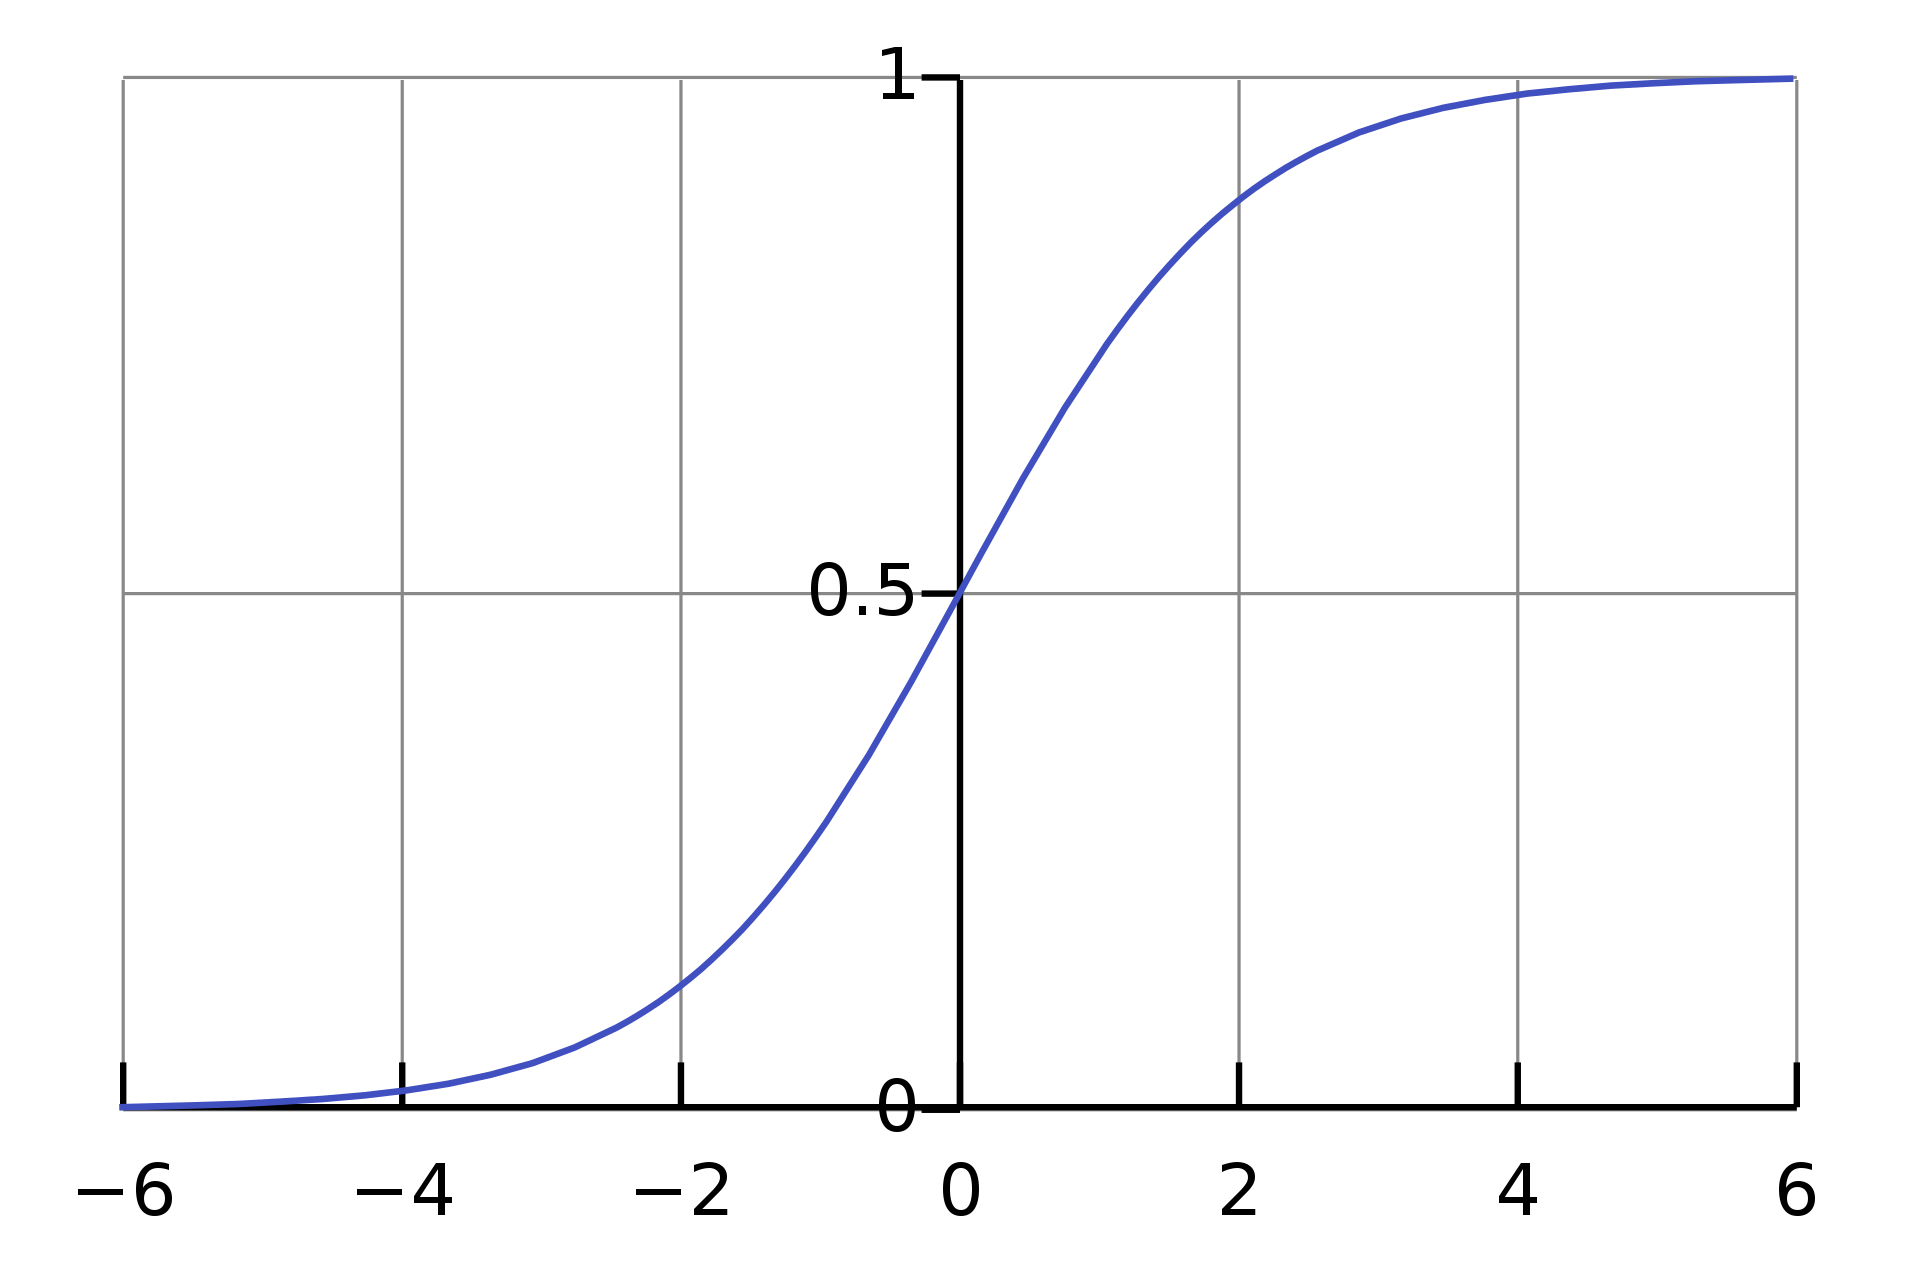
\includegraphics[keepaspectratio, width=0.36\textwidth]{img/sigmoid.png}
         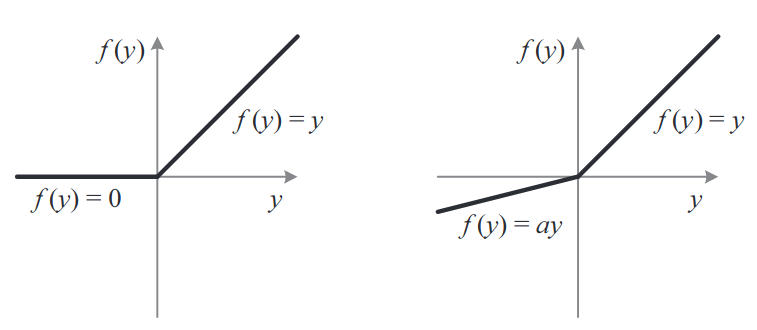
\includegraphics[keepaspectratio, width=0.63\textwidth]{img/relus.png}
      \end{center}
      \caption{
         \textbf{Left:} Sigmoid function.
         \textbf{Middle:} Rectified linear unit.
         \textbf{Right:} Rarametrized rectified linear unit~\autocite{he_delving_2015}
      }
      \label{activations}
\end{figure}

\paragraph{Normalization} layers were introduced to make training more stable and to increase the speed of convergence~\autocite{ioffe_batch_2015}.
The most commonly used normalization operations are shown in \ref{norms} and shortly described below.
\begin{itemize}
 \item batch normalization~\autocite{ioffe_batch_2015}: computes the mean and variance of \textit{a batch of inputs per channel} and normalizes the inputs to zero mean and a standard deviation of $1$.
 \item Layer normalization~\autocite{ba_layer_2016}: computes the mean and variance of \textit{ a sample across all channels} and normalizes the inputs to zero mean and a standard deviation of $1$
 \item Instance normalization~\autocite{ulyanov_instance_2017}: computes the mean and variance of a \textit{a sample across one channels} and normalizes the inputs to zero mean and a standard deviation of $1$
 \item Group normalization~\autocite{wu_group_2018}: computes the mean and variance of a \textit{a sample across a group of channels} and normalizes the inputs to zero mean and a standard deviation of $1$
\end{itemize}
\fig{img/norms.png}{norms}{Visualization of how the mean and variance is computed for each normalization operation that is used in practice.}{1}

\paragraph{Drop-out} layers are used to mask parts of the neurons in a layer in a probabilistic manner to decrease overfitting, i.e. to improve generalization~\autocite{srivastava_dropout_2014}.
Overfitting is the phenomenon that occurs when a machine learning model is trained for many epochs on the same training samples.
When unseen samples are presented the network performs significantly worse than on the training data.
A conceptual visualization of multiple dropout layers in a network is shown in \ref{dropout}.
Drop-out also improve the robustness of the NN to artifacts \& noise and serves as a passive augmentation technique, as when dropout occurs, it appears to the network as if the input has been masked randomly.
\fig{img/dropout.png}{dropout}{Abstract visualization of dropout~\autocite{srivastava_dropout_2014}.}{0.5}

\paragraph{Pooling} layers are used to reduce the dimensionality between layers or blocks of layers.
Reducing the size of the representation is essential in two ways: first, it reduces the computational costs in subsequent layers, while second it compresses the representation that was usually expanded to more channels.
The second part is closely related to convolutions, in the sense of that convolutions usually slightly reduce the spatial size of the representation while expanding the number of channels.
As the number of channels is usually increased by a factor per layer or block by a constant factor (e.g. $2$), the spatial dimension only shrinks by a factor that is smaller.
Pooling is also used to add spatial invariance, for example permutation invariance within the pixels that get pooled together~\autocite{goodfellow_deep_2016}.
To accomodate for that pooling is used.
The two most common pooling operations used in practice are MaxPooling~\autocite{zhou_computation_1988} and AveragePooling~\autocite{gholamalinezhad_pooling_nodate}.
Max pooling groups a number of pixels together and returns the maximum per group.
This is relatively sensitive to outliers but preserves strong signals in the network.
Average pooling returns the average of a group of pixels.
While it is not as sensitive to outliers, it may decrease the entropy of the signal.
A visualization of both operations in shown in~\ref{pooling}.
\fig{img/pool.png}{pooling}{Max pooling (left) and average pooling (right) visualized for single channel 2D input from the previous layer.}{0.8}

Finally, \paragraph{Skip connections} or residual connections were introduced by~\autocite{he_deep_2016} in order to reduce convergence time and imcrease accuracy.
Essentially, skip connections cause convolutional layers (in combination they are used very commonly) not to learn an unreferenced presentation but rather to extract the desired change in representation.
This is done by ``copying'' the input to a layer or a block, then performing convolution, activation and normalization and finally adding the input to the layer to the output.
Again, this encourages the convolution operation to only address the changes from the identity mapping that are beneficial to the task instead of learning to conserve the general representation of the input from the previous layer as well.
Thus they can be seen as a kind of shortcut~\autocite{he_deep_2016}.
An illustration of a skip connection in the architecture of a block is shown in \ref{skip}.
\fig{img/skip.png}{skip}{Diagram of a block in a neural net that incorporates a skip connection~\autocite{he_deep_2016}. Weight layers stand for convolution or dense layers for example.}{0.5}



\subsection{Architecture}
UNet, challenges, impact of transformers, ...

\subsection{Training}

\subsection{Image-to-Image Synthesis}

\subsection{Deep Learning in Medical Imaging}

\paragraph{pc-bSSFP \& DTI in Neuronal Networks}




\chapter{Methods}\label{\positionnumber} 
\section{The Dove Dataset}
Some stats on size 
\subsection{Participants \& Study Design}
briefly describe participants, task, scanning times (of the day)

\subsection{Recorded Sequences}
cf gais doc.
Details on acquisitions

\section{Data Processing}
requirements
\subsection{bSSFP}

\subsection{DWI}
TODO ask svenja what was done

\subsection{Augmentation}


\section{Machine Learning-based DWI Tensor estimation from bSSFP data}
MONAI, torchio, pytorch lightning. 

\subsection{Architecture}
UNet + some extra layers to fit output dim.

\subsection{Training}
Pre-training, transfer \& fine-tuning \\

Sparse data, small batch sizes. => Augmentation not enough => Pre training
\paragraph{AutoEncoder PreTraining}
As auto encoder. train autoenc for bssfp only 

\paragraph{ExtraHead Transfer and Fine tuning}
freeze autoenc, add head. transfer then unfreeze all and fine tune
Unet + extra head

\cleardoublepage
\chapter{Results}\label{\positionnumber}

\section{Direct bSSFP to DWI Tensor Training}

\section{Pre-Training \& bSSFP Transfer-Learning}

\section{Comparison of Voxel-wise to Volume-wise Regression}

\section{Modality Comparisons}
\subsection{Quantitative comparison of Quality differences between Auto-Encoding and pc-bSSFP Image to Image Translation}
\subsection{pc-bSSFP is more suitable than single-volume Structural Images}
\subsection{Phase-cycles contain relevant the Information}
\subsection{Asymmetry Index Maps distill phase-cycle Information}








\cleardoublepage
\chapter{Discussion}\label{\positionnumber}

\section{Limitations}
voxel- patch - volume pro-con\\
Statistical power \\
model size/speed \\
learned vs. closed-form/deduced/analytical transformation \\
igh frequency features and gan loss (show diff maps) \\
Augmentation \\
error propagation of denorm to scalars \\
masks \& probsegs imperfect, currently regenerated w freesurfer by svenja k \\
registration for bssfp for many subject difficult \\

\section{Future Work}
\subsection{Modular Deep Learning}
Pretrain .\\
LDM for latent translation\\
GAN \& Stable diffusion, control flow matching, latent diffusion models\\
phase cycle und miller \\
predict t2ws to establish better comparability wrt. scalars \\
multi res, multi input, multi output/foundation model \\

\subsection{Conv Transf.}
New kid on the block\\

\subsection{Neural Arch Search}
DiNTS

\chapter{Acknowledgements}
Rahel, Flo, Qi, Klaus

\cleardoublepage
\appendix
\renewcommand{\thesection}{\Alph{section}}
\chapter*{Appendix}
\addcontentsline{toc}{chapter}{Appendix}


\printbibliography




   \begin{figure}[h]
      \begin{center}
         %[keepaspectratio, width=0.45\textwidth]{img/0.jpg}
      \end{center}
      \caption{
         \textbf{A. \& B.} SNc and projections to the dorsal striatum in healthy subjects and patients with PD. 
         In the healthy subject, the SNc is still highly pigmented due to the melanin-containing dopamine-producing cells being intact.
         The SNc projects to the striatum and delivers normal amounts of DA into the basal ganglia (BG) circuit.
         If the dopamine-producing neurons undergo apoptosis, the pigmentation decreases and so does the amount of dopamine adimnistered to the striatum. 
         \textbf{C.} Photomicrographs of Lewy bodies.
      }
      \label{broad-mech}
   \end{figure}


\section{Discussion}




\end{document}
